\documentclass[11pt,a4paper,oneside,listof=totoc,headsepline,footsepline,parskip=half,numbers=noenddot,headings=standardclasses]{scrbook}
\usepackage[utf8]{inputenc}
\usepackage[english]{babel}
\usepackage{newpxtext,newpxmath}

\usepackage{fancyhdr}
\pagestyle{fancyplain}
\fancyhead{}

\usepackage{float}
\usepackage{mathtools}
\usepackage{gensymb}
\usepackage{textcomp}
\usepackage{mathrsfs}
\usepackage{siunitx}
\sisetup{range-phrase=~...~}
\usepackage{booktabs}
\usepackage{xcolor}
\usepackage{nicefrac}
%\usepackage{microtype}

%tikz stuff
\usepackage{tikz}
\usepackage{tikzscale}
\usepackage{pgfplots}
\pgfplotsset{compat=newest}
\usetikzlibrary{arrows.meta}
\usetikzlibrary{plotmarks}
\usetikzlibrary{matrix}
\pgfplotsset{compat=1.5.1}
\usepackage[list=false]{subcaption}
\usepackage[export]{adjustbox}
\usetikzlibrary{external} %externalize all tikz pictures
\tikzexternalize[optimize=false,prefix=tikz/]

%urls
\usepackage[hyphens]{url}
\def\UrlBreaks{\do\/\do-}
\usepackage[breaklinks]{hyperref}

%equation variable descriptions
%aligned:
\newenvironment{with}
{\par\vspace{\abovedisplayskip}\noindent\begin{tabular}{>{$}l<{$} @{${}:{}$} l}}
	{\end{tabular}\par\vspace{\belowdisplayskip}}
%aligned multiline
\usepackage{array,tabularx}
\newenvironment{with*}
{\par\vspace{\abovedisplayskip}\noindent
	\tabularx{\columnwidth}{>{$}l<{$} @{${}:{}$} >{\raggedright\arraybackslash}X}}
{\endtabularx\par\vspace{\belowdisplayskip}}



%%%%%%%% KIT Physik Vorlage %%%%%%%%%%%%%%%%%%%%%%%%%%%%%%%%
\usepackage[absolute,overlay]{textpos}          
\usepackage{tikz}                               
\usepackage{ifthen}                             
\usepackage[fit,breakall]{truncate}

\newcommand{\thesisauthor}{Marvin-Dennis Noll}
\newcommand{\thesistopic}{Stability improvements of the FLUTE RF supply}
\newcommand{\thesisentopic}{nix}
\newcommand{\thesislongtopic}{}
\newcommand{\thesisinstitute}{Institute for Beam Physics and Technology (IBPT)}
\newcommand{\thesisreviewerone}{Prof. Dr.-Ing. John Jelonnek (IHM)}
\newcommand{\thesisreviewertwo}{Prof. Dr. Anke-Susanne Müller}
\newcommand{\thesisadvisorone}{} % to use: enter names and uncomment in titlepg
\newcommand{\thesisadvisortwo}{}
\newcommand{\thesistimestart}{15.11.2020} % on titlepage
\newcommand{\thesistimeend}{15.05.2021} % on titlepage
\newcommand{\thesistimehandin}{15.05.2021} % on second page 'preamble'
\newcommand{\thesispagehead}{Bachelorarbeit: \thesisentopic} % page heading 
\newcommand{\changefont}[3]{\fontfamily{#1} \fontseries{#2}%
	\fontshape{#3} \selectfont}
\usepackage{vmargin}
\setpapersize{A4}
\setmarginsrb{3cm}{1cm}{3cm}{1cm}   % {leftmargin}{topmargin}{rightmargin}...
{6mm}{7mm}{5mm}{15mm}    			% {bottommargin}{headheight}{headsep}...
									% {footheight}{footskip}
\setlength{\marginparwidth}{1.5cm}
%%%%%%%%%%%%%%%%%%%%%%%%%%%%%%%%%%%%%%%%%%%%%%%%%%%%

\begin{document}
\frontmatter
%%modified by Marvin Noll (2018)
% coordinates for background border
\newcommand{\diameter}{20}
\newcommand{\xone}{-15}
\newcommand{\xtwo}{160}
\newcommand{\yone}{15}
\newcommand{\ytwo}{-253}


\begin{titlepage}
    % background border
    \begin{tikzpicture}[overlay]
    \draw[color=gray]
            (\xone mm, \yone mm)
      -- (\xtwo mm, \yone mm)
    arc (90:0:\diameter pt)
      -- (\xtwo mm + \diameter pt , \ytwo mm)
        -- (\xone mm + \diameter pt , \ytwo mm)
    arc (270:180:\diameter pt)
        -- (\xone mm, \yone mm);
    \end{tikzpicture}



    % KIT image and sign for faculty of physics
    \begin{textblock}{10}[0,0](4,2.5)
        \includegraphics[width=.25\textwidth]{kitlogo.pdf}
    \end{textblock}
    \changefont{phv}{m}{n}    % helvetica
    \begin{textblock}{10}[0,0](6,2.2)
        \begin{flushright}
            \small FAKULTÄT FÜR ELEKTROTECHNIK UND INFORMATIONSTECHNIK\\
            \Large \thesisinstitute
        \end{flushright}
    \end{textblock}



    % horizontal line
    \begin{textblock}{10}[0,0](4.2,3.1)
        \begin{tikzpicture}[overlay]
        \draw[color=gray]
                (\xone mm + 5 mm, -12 mm)
          -- (\xtwo mm + \diameter pt - 5 mm, -12 mm);
        \end{tikzpicture}
    \end{textblock}



    % begin of text part
    \changefont{phv}{m}{n}    % helvetica
    \centering



    % thesis topic (en and ge)
    \vspace*{3cm}
    \Huge\thesistopic\\
    %\huge(\thesisentopic)\\



    % author name and institute
    \vspace*{2cm}
    \Large Master thesis\\of\\
    \vspace*{1cm}
    \huge\thesisauthor\\
    \vspace*{1cm}
    \Large am \thesisinstitute



    % possible frontimage - thanks to JabberWok
    % for publishing the img under GNU Document License
    \vspace*{1.5cm}
    %\includegraphics[scale=0.08]{biospecComplete.png}\\



    % examiners (Referenten)
    \vspace*{1.5cm}
    \Large
    \begin{center}
        \begin{tabular}[ht]{l c l}
        \iflanguage{english}{Reviewer}{Referent}: 
            & \hfill & \thesisreviewerone\\
        \iflanguage{english}{Second Reviewer}{Korreferent}: 
            & \hfill & \thesisreviewertwo\\
        % uncomment if you want to provide info on your advisors
        %\iflanguage{english}{Advisor}{Betreuender Mitarbeiter}: 
        %    & \hfill & \thesisadvisorone\\
        %\iflanguage{english}{Second Advisor}{Zweiter betreuender Mitarbeiter}: 
        %    & \hfill & \thesisadvisortwo\\
        \end{tabular}
    \end{center}



    % working time
    \vspace{1cm}
    \begin{center}
        \large{{From} \thesistimestart \hspace*{0.25cm} until %
                                   \hspace*{0.25cm} \thesistimeend}
    \end{center}



    % lowest text blocks concerning the KIT
    \begin{textblock}{10}[0,0](4,16.8)
        \tiny{KIT – Die Forschungsuniversität in der Helmholtz-Gemeinschaft}
    \end{textblock}
    \begin{textblock}{10}[0,0](14,16.75)
        \large{\textbf{www.kit.edu}}
    \end{textblock}
\end{titlepage}

%\chapter*{Sperrvermerk}
\thispagestyle{empty}
Die vorliegende Bachelorarbeit mit dem Titel
\\\\
\textit{Simulation von Störungen im Signalpfad eines Magnetresonanztomographen}
\\\\ 
beinhaltet vertrauliche Daten der Firma \textit{Bruker BioSpin GmbH}. Sie darf nur vom Erst- und Zweitgutachter sowie berechtigten Mitgliedern des Prüfungsausschusses eingesehen werden. Eine Veröffentlichung und Vervielfältigung der Bachelorarbeit – auch in Teilen – ist innerhalb der Sperrfrist (bis zum 30.11.2021) untersagt. Dritten darf diese Arbeit während der Sperrfrist nur mit der ausdrücklichen Genehmigung des Verfassers und Unternehmens zugänglich gemacht werden.


\chapter*{Erklärung zur Selbstständigkeit}
\thispagestyle{empty}
Ich versichere, dass ich diese Arbeit selbstständig verfasst habe und keine %
anderen als die angegebenen Quellen und Hilfsmittel benutzt habe, die %
wörtlich oder inhaltlich übernommenen Stellen als solche kenntlich gemacht und %
die Satzung des KIT zur Sicherung guter wissenschaftlicher Praxis in der %
gültigen Fassung vom 24.05.2018 beachtet habe.\\

\vspace{1cm}

\renewcommand{\arraystretch}{0} % for spacing in the tabular environment

\begin{flushright}
	\begin{tabular}{rr}
		Karlsruhe, den \thesistimehandin, & \hspace*{5cm}\\[0mm]
		\cline{2-2}\\[2mm]    % the last line has height 2mm due
		& \thesisauthor       % to \arraystretch=0
	\end{tabular}
\end{flushright}

\vfill

\begin{flushright}
	Als Prüfungsexemplar genehmigt von\\
	\vspace{1cm}
	\begin{tabular}{rr}
		Karlsruhe, den \thesistimehandin, & \hspace*{5cm}\\[0mm]
		\cline{2-2}\\[2mm]    % the last line has height 2mm due
		& \thesisreviewerone  % to \arraystretch=0
	\end{tabular}
\end{flushright}

\renewcommand{\arraystretch}{1}

\cleardoublepage


\thispagestyle{empty}
\pagenumbering{roman}
\setcounter{page}{0}
\tableofcontents
\cleardoublepage
\pagenumbering{arabic}
\setcounter{page}{1}

\mainmatter
%\section{Evaluation of the \textit{ZX73-2500-S+} voltage dependent attenuator}

According to the datasheet, the ZX73-2500-S+ is usable over a frequency range of \SIrange{10}{2500}{\MHz}.

For the following tests, a supply voltage of \SI{3}{\V} is used.

\begin{figure}[H]
	\centering
	\includegraphics[width=\textwidth,height=0.5\textwidth]{img/full.tikz}
	\caption{Power transmission through the attenuator with different control voltages $V_{ctrl}$ (using the whole range up to the maximum allowed $V_{ctrl} \approx \SI{18}{\volt}$)}
	\label{fig:full}
\end{figure}

\begin{figure}[H]
	\centering
	\includegraphics[width=\textwidth,height=0.7\textwidth]{img/around4.tikz}
	\caption{Power transmission through the attenuator with different control voltages $V_{ctrl} = \SIrange{4}{4.15}{\volt}$}
	\label{fig:around4}
\end{figure}

\begin{figure}[H]
	\centering
	\includegraphics[width=\textwidth,height=1.5\textwidth]{img/around4_2.tikz}
	\caption{Power transmission through the attenuator with different control voltages $V_{ctrl} = \SIrange{4}{4.15}{\volt}$ (Zoomed in version of \autoref{fig:around4})}
	\label{fig:around4_2}
\end{figure}

\begin{figure}[H]
	\centering
	\includegraphics[width=\textwidth,height=0.5\textwidth]{img/vctrl.tikz}
	\caption{Relation $S_{21} = S_{21}(V_{ctrl})$ (for fixed frequency $f=\SI{3}{\GHz}$)}
	\label{fig:vctrl}
\end{figure}

\begin{figure}[H]
	\centering
	\includegraphics[width=\textwidth,height=0.5\textwidth]{img/dvctrl.tikz}
	\caption{Sensitivity $\frac{\text{d}\;S_{21}}{\text{d}V_{ctrl}}$}
	\label{fig:dvctrl}
\end{figure}

\begin{figure}[H]
	\centering
	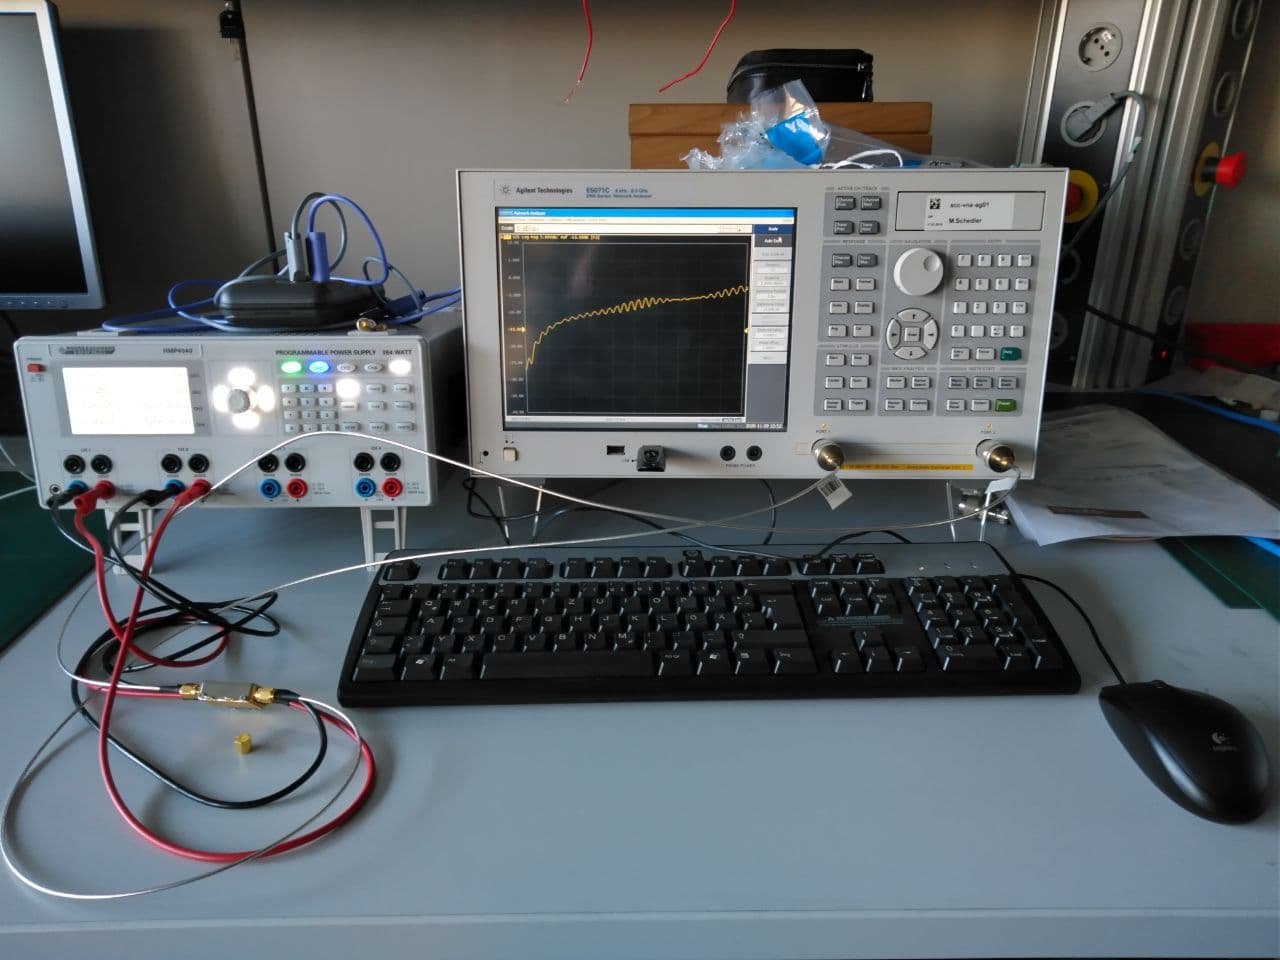
\includegraphics[width=\textwidth]{img/setup.jpg}
	\caption{The setup with power supply (left) and network analyzer (right)}
	\label{fig:setup}
\end{figure}



\chapter{Evaluation of a voltage controlled RF attenuator}
\section{Measurement setup}

\begin{figure}[H]
	\centering
	\includegraphics[]{img/atteneval/schematic.tikz}
	\caption{Measurement setup: DUT(red), RF generator/meter(blue), DC sources/ sinks(green)}
	\label{fig:atteneval-setup}
\end{figure}

\newpage
\section{Stability and noise of the DAC outputs}

\begin{figure}[H]
	\centering
	\includegraphics[width=\textwidth,height=0.5\textwidth]{img/atteneval/spec/vplus_time.tikz}
	\caption{Time signal of DAC channel 204, i.e. $V+$}
	\label{fig:vplus_time}
\end{figure}

\begin{figure}[H]
	\centering
	\includegraphics[width=\textwidth,height=0.5\textwidth]{img/atteneval/spec/vplus_spec.tikz}
	\caption{Spectrum of DAC channel 204, i.e. $V+$}
	\label{fig:vplus_spec}
\end{figure}


\begin{figure}[H]
	\centering
	\includegraphics[width=\textwidth,height=0.5\textwidth]{img/atteneval/spec/vctrl_time.tikz}
	\caption{Time signal of DAC channel 205, i.e. $V_{control}$}
	\label{fig:vctrl_time}
\end{figure}

\begin{figure}[H]
	\centering
	\includegraphics[width=\textwidth,height=0.5\textwidth]{img/atteneval/spec/vctrl_spec.tikz}
	\caption{Spectrum of DAC channel 205, i.e. $V_{control}$}
	\label{fig:vctrl_spec}
\end{figure}





\newpage
\section{Relation between $V_{control}$ and the RF attenuation}
\begin{figure}[H]
	\centering
	\includegraphics[width=\textwidth,height=0.5\textwidth]{img/atteneval/ctrl/dmm2_time.tikz}
	\caption{Control voltage $V_{control}$}
	\label{fig:vctrl_spec}
\end{figure}

\begin{figure}[H]
	\centering
	\includegraphics[width=\textwidth,height=0.5\textwidth]{img/atteneval/ctrl/pm_time.tikz}
	\caption{RF power}
	\label{fig:vctrl_spec}
\end{figure}

\begin{figure}[H]
	\centering
	\includegraphics[width=\textwidth,height=0.5\textwidth]{img/atteneval/ctrl/temp_time.tikz}
	\caption{Device temperature}
	\label{fig:vctrl_spec}
\end{figure}

\begin{figure}[H]
	\centering
	\includegraphics[width=\textwidth,height=0.6\textwidth]{img/atteneval/ctrl/ctrl.tikz}
	\caption{Relation between $V_{control}$ and RF power; showing all data points (in 60 s bins)}
	\label{fig:vctrl_spec}
\end{figure}

\begin{figure}[H]
	\centering
	\includegraphics[width=\textwidth,height=0.6\textwidth]{img/atteneval/ctrl/ctrlgroup.tikz}
	\caption{Relation between $V_{control}$ and RF power; showing data point grouped by set control voltages with a mean aggregation}
	\label{fig:vctrl_spec}
\end{figure}



\newpage
\section{Influence of the supply voltage $V+$}
\begin{figure}[H]
	\centering
	\includegraphics[width=\textwidth,height=0.5\textwidth]{img/atteneval/supp/dmm1_time.tikz}
	\caption{Supply voltage $V+$}
	\label{fig:vctrl_spec}
\end{figure}

\begin{figure}[H]
	\centering
	\includegraphics[width=\textwidth,height=0.5\textwidth]{img/atteneval/supp/pm_time.tikz}
	\caption{RF power}
	\label{fig:vctrl_spec}
\end{figure}

\begin{figure}[H]
	\centering
	\includegraphics[width=\textwidth,height=0.6\textwidth]{img/atteneval/supp/supp.tikz}
	\caption{Relation between $V+$ and RF power; showing all data points (in 30 s bins)}
	\label{fig:vctrl_spec}
\end{figure}





\newpage
\section{Influence of temperature variations $\vartheta_{case}$}
\begin{figure}[H]
	\centering
	\includegraphics[width=\textwidth,height=0.5\textwidth]{img/atteneval/temp/temp_time.tikz}
	\caption{Temperature}
	\label{fig:vctrl_spec}
\end{figure}

\begin{figure}[H]
	\centering
	\includegraphics[width=\textwidth,height=0.5\textwidth]{img/atteneval/temp/pm_time.tikz}
	\caption{RF power}
	\label{fig:vctrl_spec}
\end{figure}

\begin{figure}[H]
	\centering
	\includegraphics[width=\textwidth,height=0.6\textwidth]{img/atteneval/temp/temp.tikz}
	\caption{Relation between Temperature and RF power; showing all data points}
	\label{fig:vctrl_spec}
\end{figure}




\newpage
\section{Influence of the RF frequency}





\appendix
\pagenumbering{Roman}
\setcounter{page}{0}
\chapter{RF lab devices}

\section{Benchtop multimeters}
\subsection{Agilent 34411A}
\begin{table}[H]
	\centering
	\caption{Agilent 34411A specifications}
	\label{tab:agilent-34411A-specs}
	\begin{tabular}{ll}
		\toprule
		\textbf{Specification} & \textbf{Value}\\
		\midrule
		\multicolumn{2}{c}{DC volt}\\
		Digits & 6~\nicefrac{1}{2}\\
		Measurement method & cont integrating multi-slope IV A/D converter\\
		Accuracy (\SI{10}{\volt} range, 24 hours) & \SI{0.0015}{\percent}+\SI{0.0004}{\percent} (\si{\percent} of reading + \si{\percent} of range)\\
		Bandwidth & \SI{15}{\kHz} (typ.)\\
		
		
		\bottomrule
	\end{tabular}
\end{table}

\begin{table}[H]
	\centering
	\caption{Agilent 34411A some SCPI commands}
	\label{tab:agilent-34411A-scpi}
	\begin{tabularx}{\textwidth}{Xll}
		\toprule
		\textbf{Description} & \textbf{Example command} & \textbf{Example return}\\
		\midrule
		Read current measurement & \texttt{READ?} & \texttt{+2.84829881E+00} (\SI{2.848}{\volt})\\
		\bottomrule
	\end{tabularx}
\end{table}


\subsection{Keysight 34470A}
\begin{table}[H]
	\centering
	\caption{Keysight 34470A specifications}
	\label{tab:keysight-34470A-specs}
	\begin{tabular}{ll}
		\toprule
		\textbf{Specification} & \textbf{Value}\\
		\midrule
		\multicolumn{2}{c}{DC volt}\\
		Digits & 7~\nicefrac{1}{2}\\
		Measurement method & cont integrating multi-slope IV A/D converter\\
		Accuracy (\SI{10}{\volt} range, 24 hours) & \SI{0.0008}{\percent}+\SI{0.0002}{\percent} (\si{\percent} of reading + \si{\percent} of range)\\
		Bandwidth & \SI{15}{\kHz} (typ.)\\
		
		
		\bottomrule
	\end{tabular}
\end{table}

\begin{table}[H]
	\centering
	\caption{Keysight 34470A some SCPI commands}
	\label{tab:keysight-34470A-scpi}
	\begin{tabularx}{\textwidth}{Xll}
		\toprule
		\textbf{Description} & \textbf{Example command} & \textbf{Example return}\\
		\midrule
		Read current measurement & \texttt{READ?} & \texttt{+9.99710196E+00} (\SI{9.997}{\volt})\\
		\bottomrule
	\end{tabularx}
\end{table}

\section{Data Acquisition/Switch Unit}
\subsection{Keysight 34972A}
\begin{table}[H]
	\centering
	\caption{Keysight 34972A specifications}
	\label{tab:keysight-34972A-specs}
	\begin{tabular}{ll}
		\toprule
		\textbf{Specification} & \textbf{Value}\\
		\midrule
		\multicolumn{2}{c}{34907A (Multifunction module)}\\
		DAC range & $\pm \SI{12}{\volt}$ \\
		DAC resolution & 16 bit ($\nicefrac{\SI{24}{\volt}}{2^{16}}$ = \SI{366.21}{\micro\volt} per bit) \\
		DAC maximum current & \SI{10}{\mA} \\
		\bottomrule
	\end{tabular}
\end{table}

\begin{table}[H]
	\centering
	\caption{Keysight 34972A some SCPI commands}
	\label{tab:keysight-34972A-scpi}
	\begin{tabularx}{\textwidth}{Xll}
		\toprule
		\textbf{Description} & \textbf{Example command} & \textbf{Example return}\\
		\midrule
		Read current measurement & \texttt{READ?} & \texttt{+2.00200000E+01} (\SI{20.02}{\degreeCelsius})\\
		Set DAC voltage of ch 204 to \SI{3.1}{\volt} & \texttt{SOUR:VOLT 3.1,(@204)} & \\
		\bottomrule
	\end{tabularx}
\end{table}


\section{Oscilloscopes}
\subsection{Tektronix MSO64}
\begin{table}[H]
	\centering
	\caption{Tektronix MSO64 specifications}
	\label{tab:tektronix-MSO64-specs}
	\begin{tabular}{ll}
		\toprule
		\textbf{Specification} & \textbf{Value}\\
		\midrule
		Bandwidth & \SI{6}{\GHz} \\
		Sample rate & \SI{25}{\giga S \per\second}\\
		ADC resolution & \SI{12}{bit}\\
		DC gain accuracy (@ \SI{50}{\ohm}, >\SI{2}{\mV\per div}) & \SI{+-2}{\percent}\\
		\bottomrule
	\end{tabular}
\end{table}

\begin{table}[H]
	\centering
	\caption{Tektronix MSO64 some SCPI commands}
	\label{tab:tektronix-MSO64-scpi}
	\begin{tabularx}{\textwidth}{Xll}
		\toprule
		\textbf{Description} & \textbf{Example command} & \textbf{Example return}\\
		\midrule
		Read mean of measurement 1 (current acq.) & \texttt{MEASUrement:MEAS1:RESUlts:CURR:MEAN?} & \texttt{3.0685821787408} \\
		\bottomrule
	\end{tabularx}
\end{table}

\section{RF signal generator}
\subsection{Rohde and Schwarz SMC100A}
\begin{table}[H]
	\centering
	\caption{Rohde and Schwarz SMC100A specifications}
	\label{tab:rs-smc100a-specs}
	\begin{tabular}{ll}
		\toprule
		\textbf{Specification} & \textbf{Value}\\
		\midrule
		Frequency range & \SI{9}{\kHz} to \SI{3.2}{\GHz}\\
		Maximum power level & \SI{17}{dBm}\\
		SSB phase noise (@ \SI{1}{\GHz}, $f_o=\SI{20}{\kHz}$, $BW=\SI{1}{\Hz}$) & \SI{-111}{dBc}\\
		Level error & $<$\SI{0.9}{\dB}\\
		\bottomrule
	\end{tabular}
\end{table}

\begin{table}[H]
	\centering
	\caption{Rohde and Schwarz SMC100A some SCPI commands}
	\label{tab:rs-smc100a-scpi}
	\begin{tabularx}{\textwidth}{Xll}
		\toprule
		\textbf{Description} & \textbf{Example command} & \textbf{Example return}\\
		\midrule
		Set RF power level to \SI{10.5}{dBm} & \texttt{SOUR:POW 10.5} & \\
		Set RF frequency to \SI{3.1}{\GHz}& \texttt{SOUR:FREQ:FIX {3.1e9}} & \\
		Enable the RF output & \texttt{OUTP on} & \\
		\bottomrule
	\end{tabularx}
\end{table}

\section{RF power meter}
\subsection{HP E4419B}
\begin{table}[H]
	\centering
	\caption{HP E4419B specifications}
	\label{tab:hp-E4419B-specs}
	\begin{tabular}{ll}
		\toprule
		\textbf{Specification} & \textbf{Value}\\
		\midrule
		Digits & 4\\
		Accuracy (abs. without power sensor) & \SI{+-0.02}{\dB} \\
		\multicolumn{2}{c}{E4410? (Power sensor)}\\
		Frequency range & \\
		Power range & \\
		\bottomrule
	\end{tabular}
\end{table}

\begin{table}[H]
	\centering
	\caption{HP E4419B some SCPI commands}
	\label{tab:hp-E4419B-scpi}
	\begin{tabularx}{\textwidth}{Xll}
		\toprule
		\textbf{Description} & \textbf{Example command} & \textbf{Example return}\\
		\midrule
		Measure power on input 1 & \texttt{MEAS1?} & \texttt{+2.89435802E+000} (\SI{2.894}{dBm}) \\
		\bottomrule
	\end{tabularx}
\end{table}



\end{document}
